\chapter{Evaluation and Results}
\label{ch:evaluation_results}

\section{Introduction}
This chapter aims to provide a comprehensive analysis of all employed model order estimation methods and deep learning models.
The evaluation is predominantly conducted on the \( \DMain_{(\text{test})} \) dataset, which was introduced in~\autoref{ch:dataset_generation}.
The effect of a varying number of snapshots \( K \) on the model performance is also scrutinized in \autoref{sec:influence_num_snapshots}, where
the dataset\( \DKvar \) is employed.


\section{Overall Performances}
For an initial comparative analysis, we consider aggregated measures of accuracy, \gls{rmse}, bias, and variance to
evaluate the performance of each model order estimation method. \\
Whereas the accuracy provides the most intuitive measure of the models' performances, the \gls{rmse} provides a more
precise measure of the magnitude of the errors. The bias and variance, on the other hand, provide a more nuanced perspective
that can be interpreted as an indicator for the models' capabilities to capture the underlying features of the data and
their generalization abilities.

\begin{figure}[H]
    \centering
    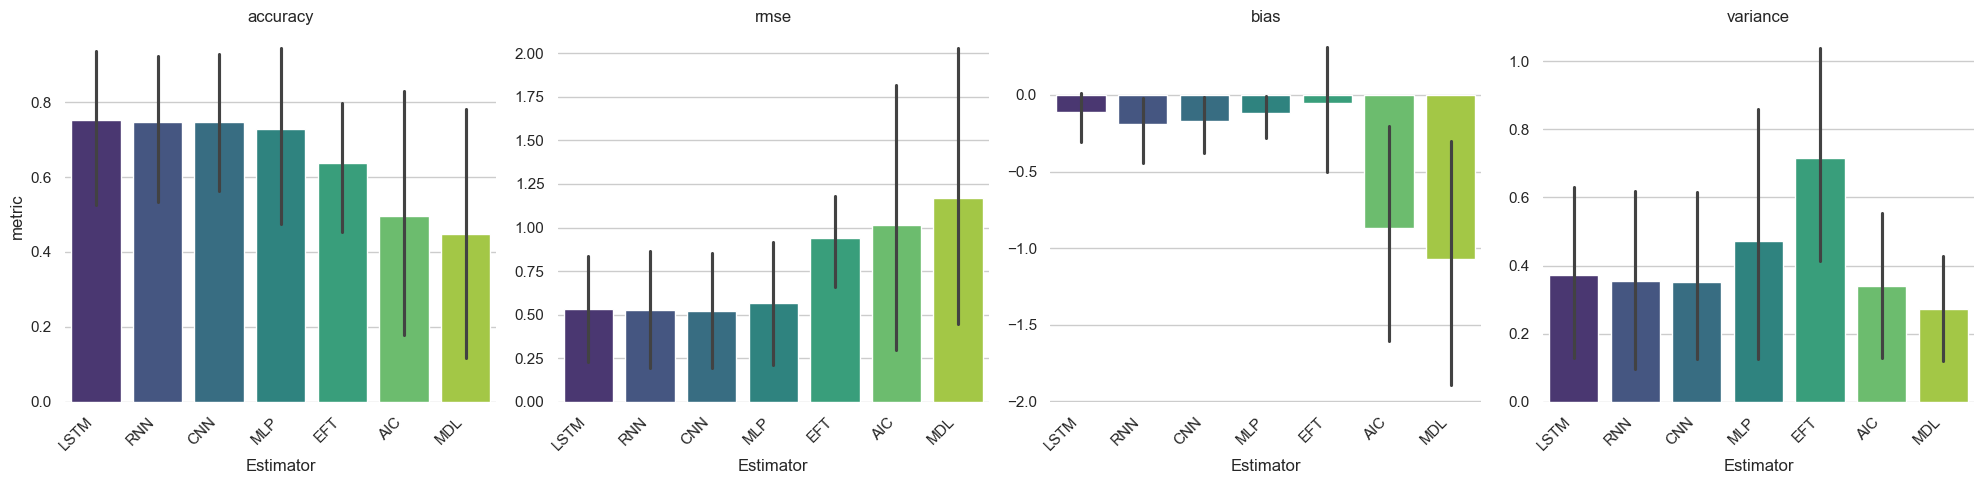
\includegraphics[width=1\textwidth]{figures/07_Evaluation/global_metrics_acc,bias,var.png}
    \caption{Accumulated accuracy, \gls{rmse}, bias, and variance of the model order estimation methods.}
    \label{fig:global_metrics}
\end{figure}
\autoref{fig:global_metrics} visually encapsulates these metrics, demonstrating a distinct advantage of the deep
learning approaches (\gls{lstm}, \gls{rnn}, \gls{cnn}, and \gls{mlp}) over the conventional
\glspl{ic} (\gls{aic} and \gls{mdl}) in terms of accuracy, \gls{rmse}, and bias.\\
The \gls{eft} demonstrates an intermediate performance, outpacing traditional methods while trailing
behind deep learning models in terms of accuracy and RMSE but exhibits the highest overall
variance. \\
The thin black lines on the bar graphs within~\autoref{fig:global_metrics} represent the 95\% confidence intervals
for each metric. These intervals are computed by collating the metrics for all true model orders \(N\) and then averaging
them across the entire dataset. \\

The contents of \autoref{fig:global_metrics} are gathered in \autoref{tab:global_metrics}, which also includes the
relative changes in metrics with respect to the most accurate model, the \gls{lstm}.
The green and red boxes highlight the best and worst performers for each metric. \\

\begin{table}[H]
    \centering
    \caption{Performance Comparison of Estimators on \( \DMain_{(\text{test})} \)}
    \label{tab:global_metrics}
    \begin{tabular}{@{}lcccccccc@{}}
    \toprule
    & \multicolumn{2}{c}{Accuracy} & \multicolumn{2}{c}{RMSE} & \multicolumn{2}{c}{Bias} & \multicolumn{2}{c}{Variance} \\
    \cmidrule(lr){2-3} \cmidrule(lr){4-5} \cmidrule(lr){6-7} \cmidrule(lr){8-9}
    Estimator & \( \nu \) & \( \%\Delta \) & \( \nu \) & \( \%\Delta \) & \( \nu \) & \( \%\Delta \) & \( \nu \) & \( \%\Delta \) \\
    \midrule
    LSTM  & \gnbx{0.7520} & - & 0.5324 & - & -0.1130 & - & 0.3721 & - \\
    RNN   & 0.7467 & -0.7023 & 0.5250 & -1.403 & -0.1874 & 65.79 & 0.3540 & -4.858 \\
    CNN   & 0.7465 & -0.7372 & \gnbx{0.5195} & -2.421 & -0.1667 & 47.49 & 0.3522 & -5.346 \\
    MLP   & 0.7276 & -3.251 & 0.5675 & 6.589 & -0.1156 & 2.275 & 0.4716 & 26.73 \\
    EFT   & 0.6363 & -15.39 & 0.9399 & 76.52 & \gnbx{-0.0542} & -52.01 & \rdbx{0.7173} & 92.76 \\
    AIC   & 0.4959 & -34.06 & 1.0120 & 90.07 & -0.8701 & 669.8 & 0.3414 & -8.252 \\
    MDL   & \rdbx{0.4476} & -40.49 & \rdbx{1.1697} & 119.7 & \rdbx{-1.0721} & 848.6 & \gnbx{0.2711} & -27.14 \\
    \bottomrule
    \end{tabular}
\end{table}

While all estimators exhibit some bias towards underestimating the model order, the deep learning models and the \gls{eft}
show a clear advantage over the \glspl{ic} by exhibiting an up to eight times lower bias.
The seemingly low variance of the traditional \glspl{ic} should not be mistaken for a superior performance, since
the extremely high bias of the \gls{aic} and \gls{mdl} is a strong indicator of their inability to accurately estimate the
model order in plenty of scenarios. \\
High bias is usually a strong indicator of a model's inability to capture the underlying features to make accurate predictions~\cite{biasVariance}.

In terms of overall performance, the \gls{cnn} is identified as the most balanced model, demonstrating the second-lowest
bias, the lowest RMSE, as well as the lowest variance among the deep learning models. While a significant portion of the
neural networks' errors being attributed to variance might initially suggest potential overfitting, further analysis in
subsequent sections offers a more refined perspective on this potentiality.

\subsubsection{Further Considerations with Respect to the Deep Learning Models}
\label{subsub:considerations_nn}

Delving deeper into the performance specifics of the deep learning models,~\autoref{tab:global_metrics:nn}
reveals the details of the neural networks' training outcomes and computational complexities.

\begin{table}[H]
    \centering
    \caption{Further Metrics of the Neural Networks on \( \DMain \).}
    \label{tab:global_metrics:nn}
    \begin{tabular}{lccccccccc}
        \toprule
        & \multicolumn{4}{c}{\( \meanLossCE \) } & \multicolumn{2}{c}{\#MACs / \(10^3\)}& \multicolumn{2}{c}{\#Params / \(10^3\)} & \multicolumn{1}{c}{\#Epochs}  \\
        \cmidrule(lr){2-5} \cmidrule(lr){6-7} \cmidrule(lr){8-9} \cmidrule(lr){10-10}
         & \multicolumn{2}{c}{Train} & \multicolumn{2}{c}{Val} & & & & & \\
        \cmidrule(lr){2-3} \cmidrule(lr){4-5}
        Model& \( \nu \) & \( \%\Delta \) & \( \nu \) & \( \%\Delta \) & \( \nu \) & \( \%\Delta \) & \( \nu \) & \( \%\Delta \) & \( \nu \)  \\
        \midrule
        LSTM    & 0.527 & -     & 0.525 & -    & 50.54  & -     & 6.4 & -     & 8 \\
        RNN     & 0.538 & \rdbx{2.18}  & 0.540 & \rdbx{2.97} & 13.18  & \gnbx{-73.9} & 2.6 & \gnbx{-59.4} & 9 \\
        CNN     & 0.542 & \rdbx{2.92}  & 0.535 & \rdbx{1.89} & 9.24   & \gnbx{-81.7} & 2.7 & \gnbx{-57.8} & 4 \\
        MLP     & 0.562 & \rdbx{6.69}  & 0.569 & \rdbx{8.46} & 2.62   & \gnbx{-94.8} & 2.5 & \gnbx{-60.9} & 8 \\
        \midrule[0.1pt]
        GRU     & 0.526 & \gnbx{-0.19} & 0.527 & \rdbx{0.44} & 9.36   & \gnbx{-81.5} & 1.9 & \gnbx{-70.3} & 7 \\
        \bottomrule
    \end{tabular}
\end{table}

The analysis reveals that the training and validation losses across all neural networks do not exhibit a significant
difference. This observation suggests that the high variance noted may not solely stem from model overfitting.
Instead, it could be attributed to the inability of the input data, the eigenvalues \( \bfL \), to encode
the desired information in certain scenarios, as initially hypothesized by~\cite{barthelme21sub} and formally introduced
in~\autoref{sec:challenges_moe}. This perspective challenges the overfitting hypothesis by highlighting data limitations
as a contributing factor to model performance issues.

Moreover, the observation that \( \meanLossCETrain < \meanLossCEVal \) for the \gls{cnn} can be attributed to the
application of regularization techniques, such as dropout and L2 regularization, exclusively during training.
These techniques are designed to mitigate overfitting by penalizing model complexity and encouraging simpler models that
generalize better to unseen data. The fact that these regularization measures are implemented only during training further
supports the argument against the overfitting hypothesis, suggesting that the model's design actively seeks to balance
bias and variance.

The \gls{cnn} model's quick convergence, achieved in just four epochs before meeting the early stopping criterion,
indicates efficient learning and optimization.
This rapid convergence is likely due to an optimized learning rate and effective gradient smoothing through layer
normalization. \\
However, this efficiency also implies that learning rate scheduling, which could further refine model performance over a
more extended training period, was not fully leveraged. \\
A logical consequence would be the adaptation of the employed datasets, so that the training process could be extended
over more epochs, as will be discussed in~\autoref{subsub:training_data}.

The \gls{mlp} model, while incorporating layer normalization to aid in training stability, might have been hindered by
an overly aggressive learning rate setting, with \( \alpha = 0.005 \). This high learning rate potentially contributed to
a less stable training process. \\
While the \gls{mlp} architecture demonstrates the lowest computational complexity in terms of \glspl{mac}, its performance
falls short of the other models. However, the performance gap might not be as significant if the skip connection had not
been omitted, as discussed in~\autoref{sub:mlp_architecture}. This adjustment would increase the \gls{mlp}'s parameter
count to around \( 2.75 \times 10^3 \).

The \gls{rnn} architecture, characterized by its relatively low parameter count, stands out as an ideal candidate for
\gls{fpga} implementations. This suitability stems from its low parameter count, which is a more critical factor than the number of \glspl{mac} in
determining the computational cost of hardware implementations. \\
Furthermore, recurrent architectures possess the largest unexplored potential and have parameter spaces that are arguably
the most amenable to pruning, as highlighted in~\autoref{subsub:future_improvements_rnn}.

The late realization of the disproportionate computational complexity, resulting from the use of a deep \gls{rnn} rather
than a shallow, single-layer architecture, led to a concise evaluation of the \gls{gru} architecture, as included
in~\autoref{tab:global_metrics:nn}. \\
Without any further optimization, the \gls{gru} architecture demonstrates a competitive performance, with a test accuracy of \( 0.76 \).
Unlike the \gls{rnn} and the \gls{lstm}, the \gls{gru} architecture features a shallow design and a hidden state comprising
only ten units. Given the data in \autoref{tab:global_metrics:nn}, these characteristics arguably render the \gls{gru}
architecture the most efficient model, thus making it the most suitable candidate for further optimization and deployment on \glspl{fpga}.

An easily identifiable trend is the marginal performance differences between the deep learning models. This observation
suggests that the models' performance might be asymptotically converging to a hard limit, which is inherent to all
eigenvalue-based model order estimation methods. \\


\section{Confusion Matrices - Influence of the Model Order}
\label{sec:confusion_matrices}
This section aims to provide a more detailed analysis of the model order estimation methods' performances by considering
the influence of the true model order \( N \) on the efficacy of the estimators. \\
Utilizing confusion matrices, we can provide a more nuanced perspective on the performance of the \gls{moe} methods by
considering specific tendencies in the predictions of each estimator. \\
The employed confusion matrices are normalized row-wise, such that the sum of prediction likelihoods for each true model
order \( N \) is equal to one.

\subsubsection{Algorithmic Estimators}

\begin{figure}[H]
    \centering
    \subfloat[]{{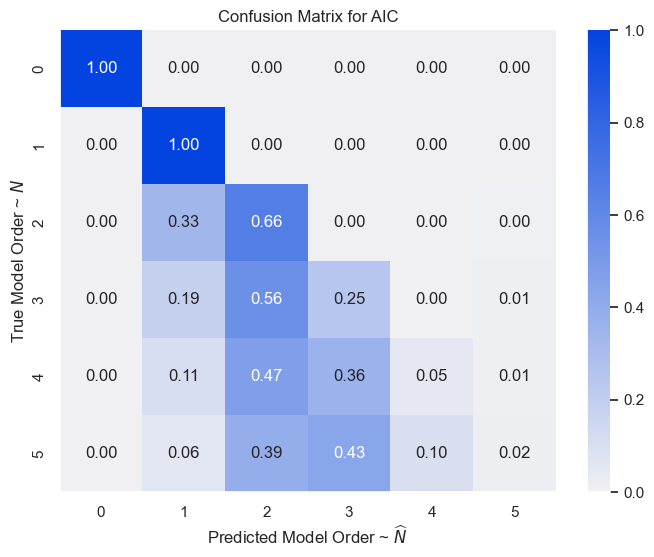
\includegraphics[width=0.31\textwidth]{figures/07_Evaluation/confusion_matrix/aic.png}}}
    \hfill
    \subfloat[]{{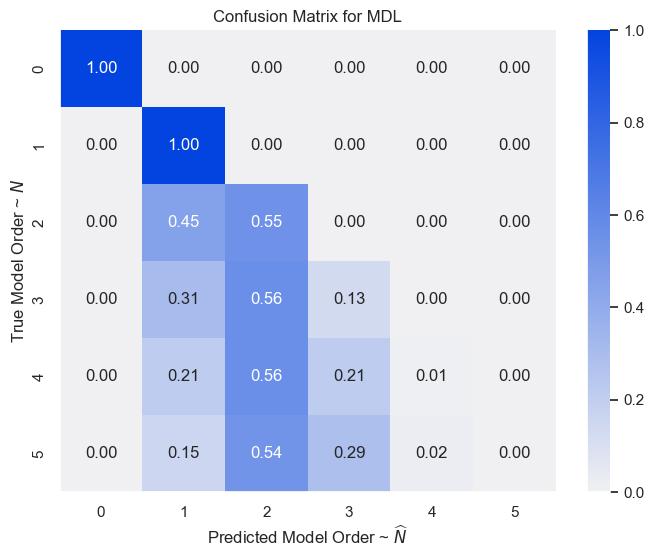
\includegraphics[width=0.31\textwidth]{figures/07_Evaluation/confusion_matrix/mdl.png}}}
    \hfill
    \subfloat[]{{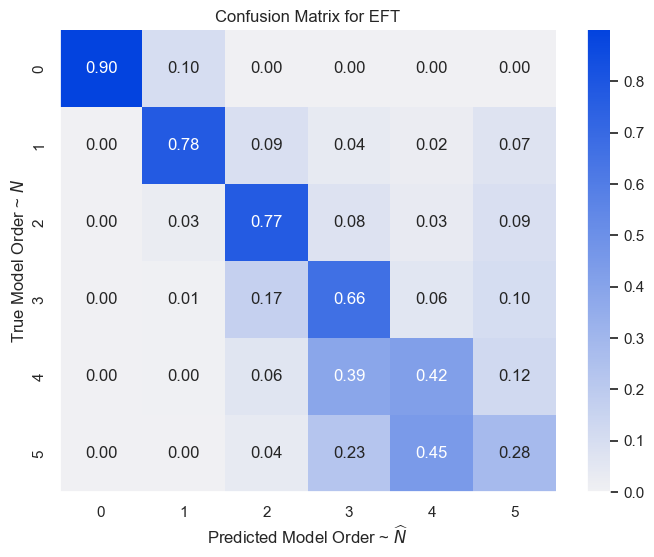
\includegraphics[width=0.31\textwidth]{figures/07_Evaluation/confusion_matrix/eft.png}}}
    \caption{Confusion matrices of the \glspl{ic}: AIC (a), MDL (b), and the EFT (c).}
    \label{fig:method_conf_matrices}
\end{figure}

\autoref{fig:method_conf_matrices} illustrates a clear tendency of the conventional criteria towards underestimating
the model order, diverging from existing literature where these criteria have been shown to overestimate model order
for \emph{coherently} constructed covariance matrices~\cite{barthelme2020}. \\
These findings furthermore explain why the \gls{mdl} is the worst performing model order estimation method, when being
evaluated on the \( \DMain_{(\text{test})} \) dataset: The \gls{mdl}'s penalty term reduces its bias towards overestimation in
fully sampled scenarios~\cite{eft}, but increases the already existing bias towards underestimation in sub-sampled scenarios. \\
Notably, when the true model order \(N\) exceeds the number of RF chains (\(N > L = 3\)), the theoretical soundness of
AIC and MDL is challenged, supporting claims made in recent studies~\cite{barthelme21sub} about their inapplicability
in the context of sub-sampled covariance matrices.

The \gls{eft} on the other hand demonstrates a notable ability to differentiate between \( N \leq L \) and \( N > L \), suggesting a
superior performance in scenarios where the model order is less than or equal to the number of available RF chains. \\
Despite this, EFT exhibits a slight overestimation bias for \( \NPred = 5 \), indicating a tendency towards false
positives in case of \( N > 0 \). Furthermore, it fails more often to predict samples with \( N \leq 1 \) correctly, which
are virtually always correct when the classical \glspl{ic} are employed. \\

\subsection{Neural Network Models Analysis}
\label{sub:nn_conf_matrices}

\begin{figure}[H]
    \centering
    \subfloat[]{{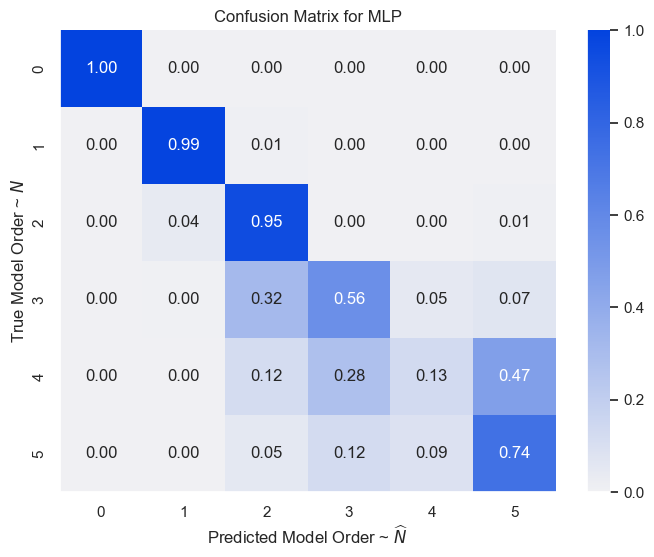
\includegraphics[width=0.48\textwidth]{figures/07_Evaluation/confusion_matrix/mlp.png}}}
    \hfill
    \subfloat[]{{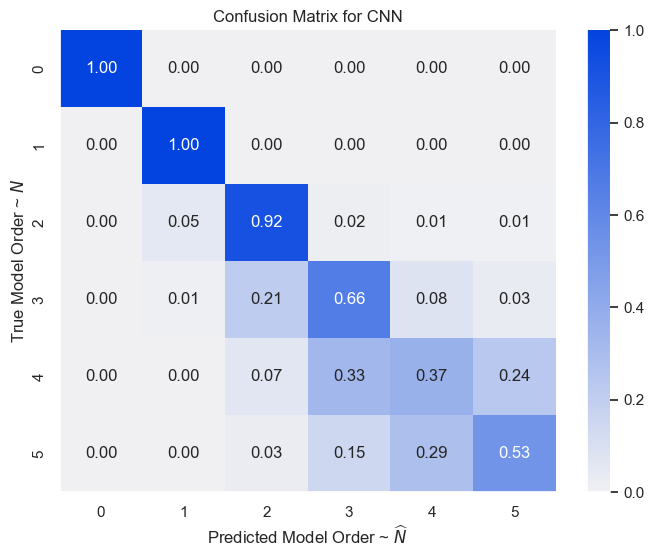
\includegraphics[width=0.48\textwidth]{figures/07_Evaluation/confusion_matrix/cnn.png}}}
    \\
    \subfloat[]{{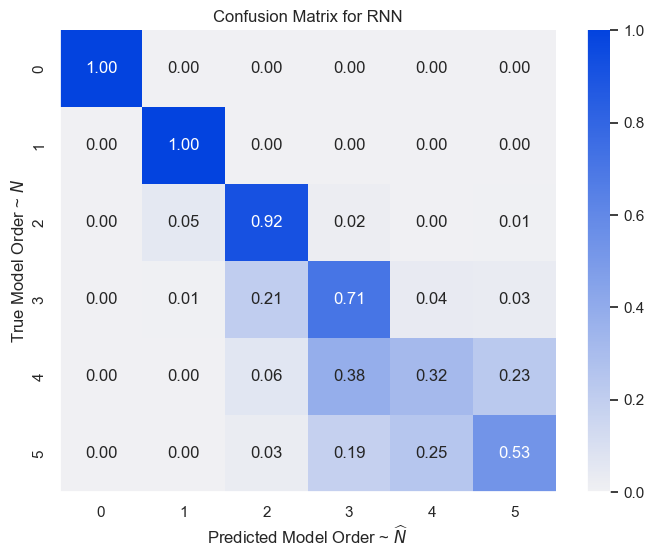
\includegraphics[width=0.48\textwidth]{figures/07_Evaluation/confusion_matrix/rnn.png}}}
    \hfill
    \subfloat[]{{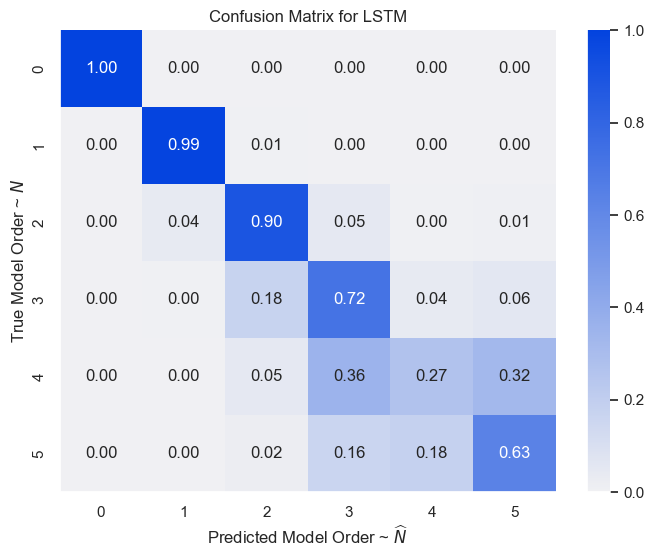
\includegraphics[width=0.48\textwidth]{figures/07_Evaluation/confusion_matrix/lstm.png}}}
    \caption{Confusion matrices of the neural networks: MLP (a), CNN (b), RNN (c), LSTM (d).}
    \label{fig:network_conf_matrices}
\end{figure}

As \autoref{fig:network_conf_matrices} shows, neural networks generally perform well when estimating lower model
orders (\( N \leq 3 \)). However, challenges arise with higher orders (\( N = 4 \) and \( N = 5 \)), where predictions
become less distinct. \\
This observation provides further evidence for the breakdown of the subspace decomposition, as claimed in~\cite{barthelme21sub}.

Despite having lower overall variances than the feed forward \gls{dnn}, the other three networks' exhibit a nearly uniform distribution of the
prediction likelihoods \( \Pr(\NPred=4|N=3) \approx \Pr(\NPred=4|N=4) \approx \Pr(\NPred=4|N=5) \) for \( N = 4 \).\\
This uniform distribution of predictions for \( N = 4 \) may suggest that a reasonable model order estimation
model order estimation, based on a single sample without prior knowledge of the statistical distribution,
might be inherently impossible.
This statement can be expressed as a hypothesis test, where the null hypothesis \( \mathcal{H}_0 \) is that the
prediction is independent of the eigenvalues \( \bfL \) of the sub-sampled covariance matrix \( \bfL \) and solely a function
of the statistics captured form the dataset and parametrized by the model weights \( \bfm{\omega} \). The alternative
hypothesis \( \mathcal{H}_a \) is that the prediction is still dependent on the information encoded in \( \bfL \).

\begin{equation}
    \Pr(\NPred|N>3) =
    \begin{cases}
    f(\bfL, \DTrain|N, K, \bfm{\Theta}; \bfm{\omega}), & \text{under } \mathcal{H}_0\\
    g(\DTrain|N, K, \bfm{\Theta}; \bfm{\omega}), & \text{under } \mathcal{H}_a
    \end{cases}
    \label{eq:pred_hypothesis}
\end{equation}

Interestingly, for \( N = 5 \), there is a discernible skew towards accurate predictions, contradicting the uniformity
observed for \( N = 4 \). This behavior would be in favor with the alternative hypothesis \( \mathcal{H}_a \) in~\autoref{eq:pred_hypothesis}
and may present an opportunity for refining prediction strategies through the implementation rule based on the observed
logits \( \bfm{z} \) of the neural networks, as formalized in~\autoref{eq:pred_rule}.

\begin{equation}
    \text{Choose } \NPred = \begin{cases}
    4, & \text{if logits } \bfm{z} \text{ for } \NPred \in \{3,4,5\} \text{ are uniformly distributed} \\
    5, & \text{if a bias towards } \NPred = 5 \text{ is present and } \bfm{z}_3 \approx \bfm{z}_4.
\end{cases}
\label{eq:pred_rule}
\end{equation}

However, further statistical analysis of the logits would clearly be necessary to confirm the feasibility of this approach since
a transfer of the observed prediction likelihoods on a population-wide scale to the logits in single samples might not be
valid.

Depending on the application, it might also be worthwhile to consider a merger of the classes \( N = 4 \) and \( N = 5 \) into a single class \( N > 3 \).
This would dramatically increase the prediction accuracy of the neural networks, might allow for further simplifications of
the network architectures, and would be a logical consequence of the theoretical assumptions that the subspace decomposition
loses its validity for \( N > 3 \). \\
Furthermore, this reformulation of the task might be a more meaningful approach to the problem, given that the claims made
in~\cite{barthelme21sub} suggest that the subspace decomposition is inherently flawed for \( N > 3 \), which would render
the application of \gls{music} -- even with a correct model order estimate -- meaningless.


\section{Influence of the SNR and SIR}
\label{sec:influence_snr_sir}

The impact of the \gls{snr} and \gls{sir} is pivotal in the realm of \gls{doa} and \gls{moe}. As the strength of the
signal relative to noise and interference directly affects the eigenvalues \( \bfm{\lambda} \), it is imperative to
understand how \gls{snr} and \gls{sir} influence the performance of model order estimation methods as well as the
practical applicability of any eigenvalue-based method. The following subsections provide an analysis of the influence's
of \( \SNRmin \), \( \SIR \), and \( \SNRmax \) and will yield further empirical evidence regarding the validity of the
hypothesis defined in~\autoref{eq:pred_hypothesis}.\\
The following effects must be considered with caution, given that extreme values of \( \SNRmin \), \( \SNRmax \), and
\( \SIR \) are significantly more likely to occur in scenarios with a higher model order, since the individual \( \SNR_i \)
for \( i \in \{0, \ldots, N\} \) are independently drawn from a uniform distribution \( \mathcal{U}(l,u) \),
where \( l \) and \( u \) are the lower and upper bounds, respectively.\\

Additionally, the definition of SIR inherently necessitates the presence of more than one signal source to hold significance,
which means that the overall accuracy in terms of \( \SIR \) is inherently lower than the accuracy in terms of \( \SNR \).
Although it's challenging to completely eliminate the profound influence of the model order on the subsequent analysis,
we provided a brief discussion on how the model order \( N \) shapes the density estimates of \( \SNRmin \), \( \SNRmax \), and \( \SIR \). \\
These correlations between the model order \( N \) and the \gls{snr} and \gls{sir} in context of the utilized datasets
have been discussed in~\autoref{subsub:snr_sir_distrib} and should be taken into account when interpreting the following
results. \\
To simplify the interpretation of these interactions,~\autoref{app:sec:FurtherMOE} provides further density estimates of
the \gls{snr} and \gls{sir} for each method, differentiating color-wise between the true, under-, and overestimated model orders
and splitting the results into different plots for cases where \( N \leq 3 \) and \( N \leq 5 \).

We will begin with a comparative analysis of all \gls{moe} methods and neural networks before providing a more detailed
analysis of the influence of \( \SNRmin \), \( \SIR \), and \( \SNRmax \) through a separation of the model orders into
individual traces in each subplot.

\subsection{Signal-to-Interference Ratio}
\label{subsec:sir}

Considering the density estimates of the \gls{sir} for the different model orders \( N \) in~\autoref{fig:sir_pdf}, it is
obvious that the \( \SIR \) still holds a significant influence on the performance of the model order estimation methods.

\begin{figure}[H]
    \centering
    \subfloat{{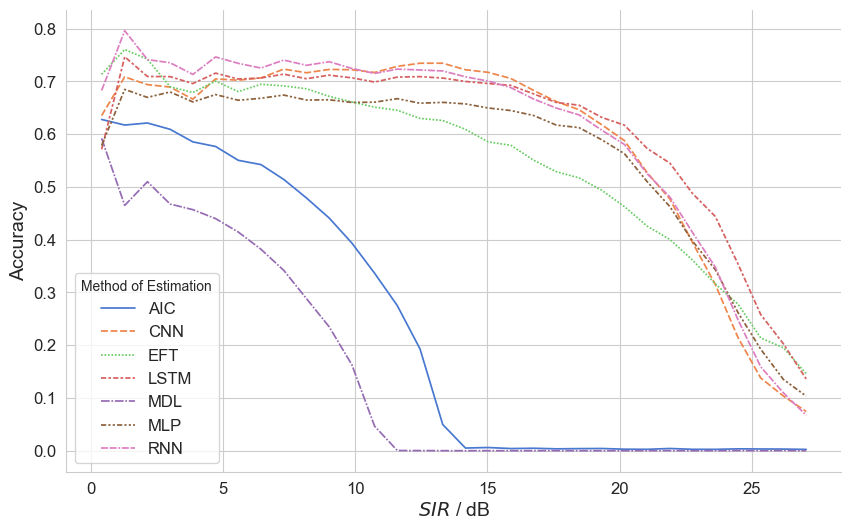
\includegraphics[width=0.5\textwidth]{figures/07_Evaluation/snr_sir/sir_acc_all.png} }}%
    \subfloat{{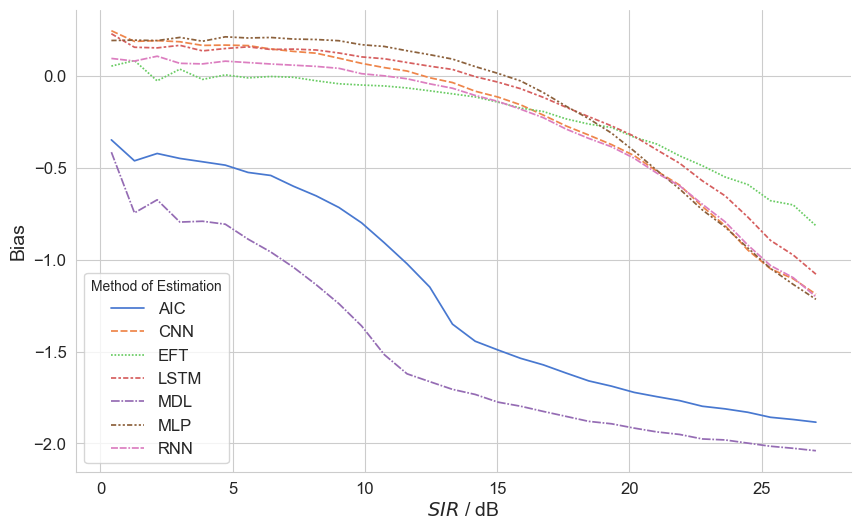
\includegraphics[width=0.5\textwidth]{figures/07_Evaluation/snr_sir/sir_bias_all.png} }}%
    \caption{Accuracy (a) \& bias (b) against \( \SIR \).}%
    \label{fig:sir_all_acc_bias}
\end{figure}

At high \gls{sir} levels, the disparity between signal eigenvalues may obscure the relative gap separating the smaller
signal eigenvalues \( \bfL_S \) from the noise eigenvalues \( \bfL_{\eta} \).
Hence, an underestimation of the
model order is more likely to occur in high \gls{sir} scenarios.

\subsection{Minimum SNR}
\label{subsec:min_snr}
Conversely, low \gls{snr} scenarios present a challenge where the
intrinsic variance within noise eigenvalues can render the distinction between the lower signal eigenvalues and noise eigenvalues untenable,
leading to overestimation of the model order when \( \SNRmin \) through false negatives when \( \SNRmin \) is low. \\
The dependence on the true model order is evident in the conventional \glspl{ic}'s extreme correlation with \( \SNRmin \) --
as \( \SNRmin \) increases, the likelihood of facing higher model orders decreases. \\


\begin{figure}[H]
    \centering
    \subfloat{{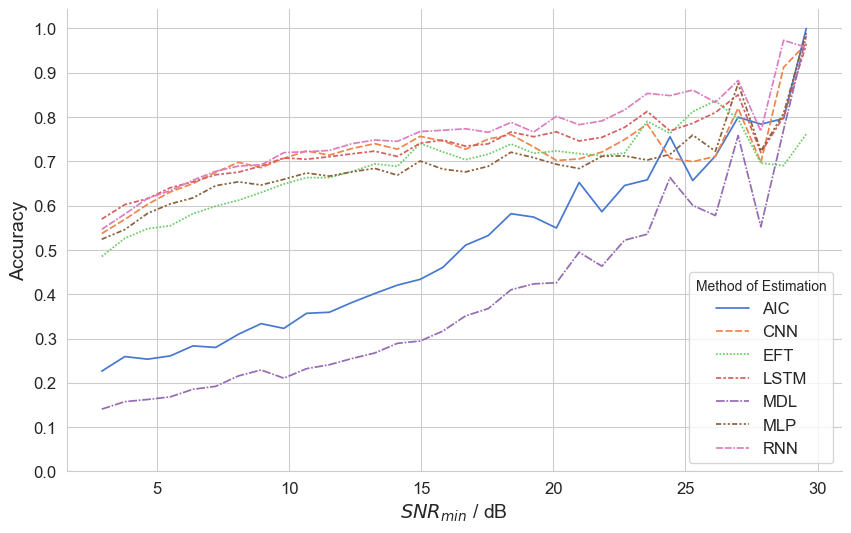
\includegraphics[width=0.5\textwidth]{figures/07_Evaluation/snr_sir/snr_min_acc_all.png}}}%
    \subfloat{{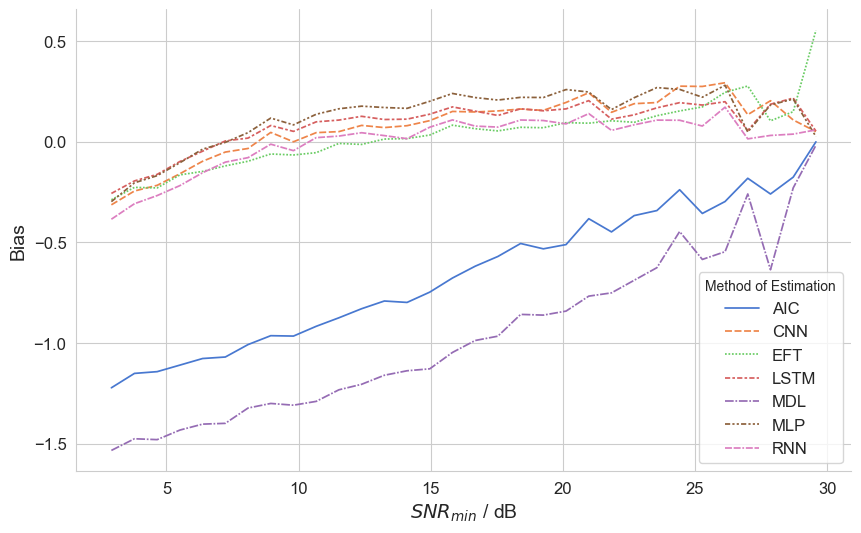
\includegraphics[width=0.5\textwidth]{figures/07_Evaluation/snr_sir/snr_min_bias_all.png}}}%
    \caption{\( \meanAccTest \) (a) \& bias (b) against \( \SNRmin \).}%
    \label{fig:snr_min_all_acc_bias}
\end{figure}

What might appear being a clearly identifiable causal relationship between \( \SNRmin \) and the performance of the estimators,
is in fact a more complex correlation, higher \( \SNRmin \) are significantly more likely to occur in scenarios with a lower
model order --~\autoref{subsub:snr_sir_distrib}.


\subsection{Maximum SNR}
\label{subsec:max_snr}

\begin{figure}[H]
    \centering
    \subfloat{{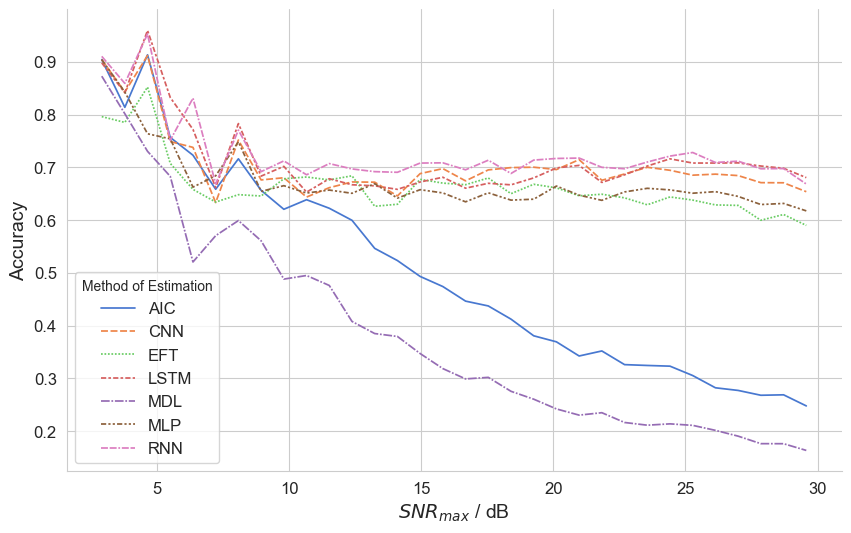
\includegraphics[width=0.5\textwidth]{figures/07_Evaluation/snr_sir/snr_max_acc_all.png} }}%
    \subfloat{{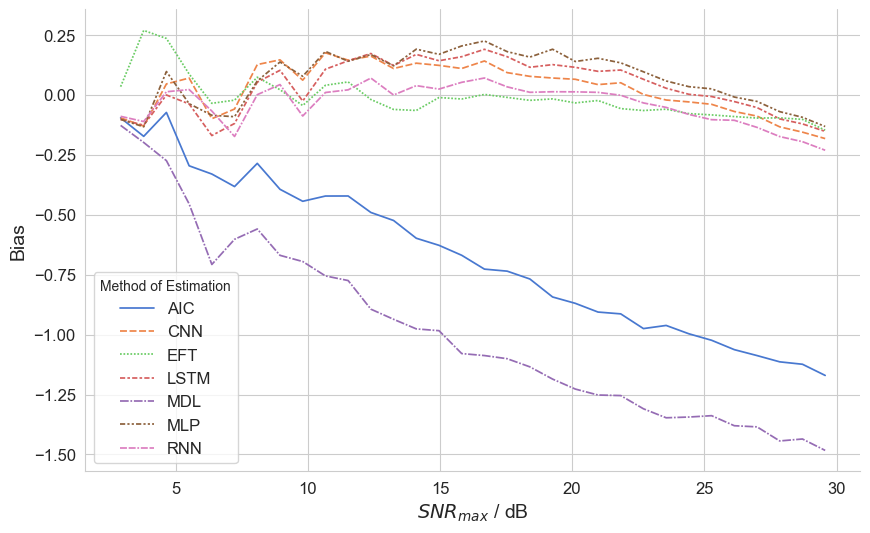
\includegraphics[width=0.5\textwidth]{figures/07_Evaluation/snr_sir/snr_max_bias_all.png} }}%
    \caption{\( \meanAccTest \) (a) \& bias (b) against \( \SNRmax \).}%
    \label{fig:snr_max_all_acc_bias}
\end{figure}

At high \gls{snr} levels, the limited numerical precision can lead to problems due to restricted dynamic ranges,
resulting in poor noise resolution. This issue becomes more pronounced with an increased number of snapshots \( K \),
as it leads to the accumulation of numerical errors when computing the sampled covariance matrix by averaging over the
\( K \) snapshots.\\
This effect significantly impacts practical applications; however, it is unlikely that numerical effects have as severe
an influence on the eigenvalues \( \bfL \) in the utilized simulation environment. \\
However, as depicted in~\autoref{fig:snr_max_noise_var}, the distribution of the noise eigenvalues \( \bfL_{\eta} \) is
influenced by \( \SNRmax \) in a way that can neither be explained by the data model nor the correlation with the model
order \( N \), which also heavily influences the distribution of the noise eigenvalues.
The latter argument is supported by the observation that the distribution of the noise eigenvalues \( \bfL_{\eta} \) does
not exhibit a complementary behavior with respect to the \( \SNRmin \).

\begin{figure}[H]
    \centering
    \subfloat{{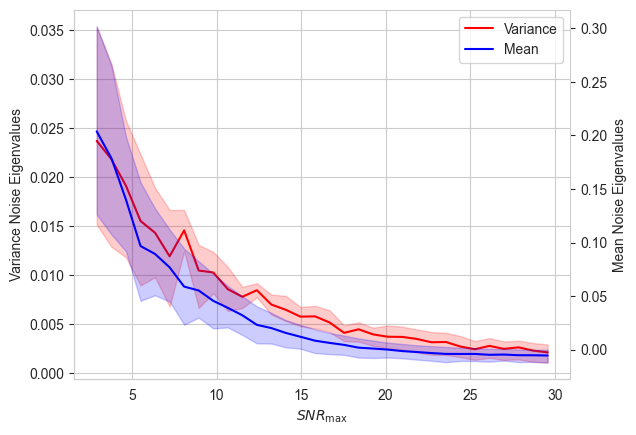
\includegraphics[width=0.45\textwidth]{figures/07_Evaluation/snr_sir/mean_var_noise_snr_max.png} }}%
    \subfloat{{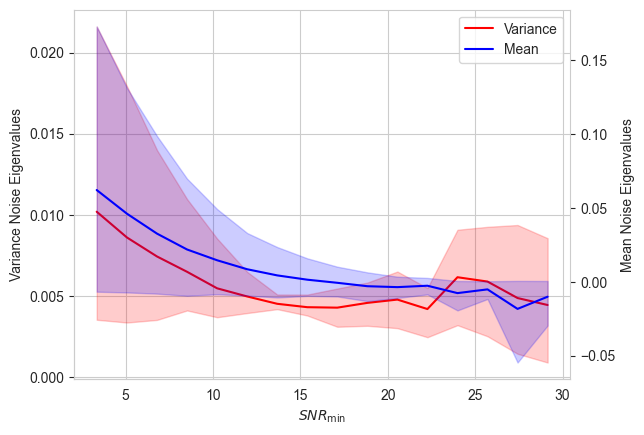
\includegraphics[width=0.45\textwidth]{figures/07_Evaluation/snr_sir/mean_var_noise_snr_min.png} }}%
    \caption{Mean (blue) and variance (red) of \( \bfL_{\eta} \) against \( \SNRmax \) (a) and \( \SNRmin \) (b).}%
    \label{fig:snr_max_noise_var}
\end{figure}

The low tendency of the neural networks towards underestimation of the model order for low \( \SNRmax \) levels is an expected
behavior, as this means that the relative differences between the signal and noise eigenvalues is less pronounced.


\paragraph{Concluding Remarks}
The graphical analysis presented in Figures~\ref{fig:sir_all_acc_bias},~\ref{fig:snr_min_all_acc_bias},and~\ref{fig:snr_max_all_acc_bias}
highlights the varying performance across different \gls{snr} and \gls{sir} conditions.
In all scenarios, deep learning approaches like \gls{lstm} and \gls{cnn} generally demonstrate robustness against \gls{snr}
and \gls{sir} variations, whereas traditional criteria like \gls{aic} and \gls{mdl} exhibit a stronger correlation with these parameters.
The \gls{eft} holds its ground, only marginally leading behind the deep learning models in terms of accuracy.

\subsection{Individual Evaluations}

The following figures provide a more detailed individual analysis of the influence of \( \SNRmin \), \( \SIR \), and \( \SNRmax \) through
a separation of the model orders into individual traces in each subplot.
These figures provide a \( 3 \times 3 \) grid of subplots, where each subplot depicts the accuracy, bias, and variance
of the model order estimation methods for a specific model order \( N \) given \( \SNRmin \), \( \SIR \), and \( \SNRmax \).

\subsubsection{Algorithmic MOEs}
\begin{figure}[H]
    \centering
    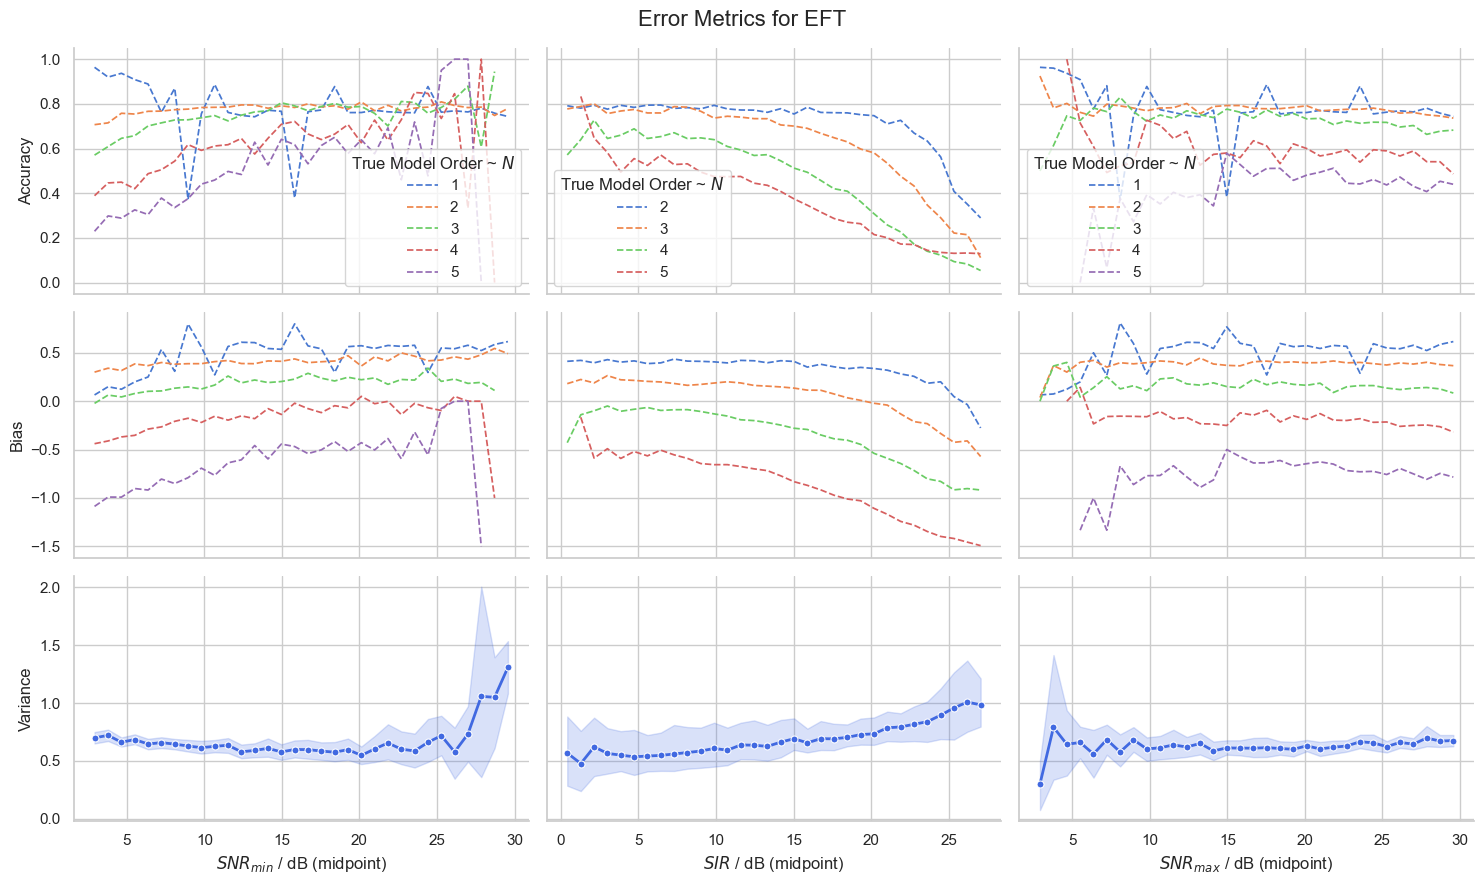
\includegraphics[width=\textwidth]{figures/07_Evaluation/snr_sir/eft_3x3.png}
    \caption{Accuracy, bias, and variance of the \gls{eft} given \( \SNRmin \), \( \SIR \) \& \( \SNRmax \).}
    \label{fig:eval_grids/eft}
\end{figure}
The incontinuity of the \gls{eft}'s accuracy and bias for \( N = 1 \) in particular, is another indicator that either the algorithm
was not implemented correctly, that the employed thresholds were not correctly chosen. \\
Another notable observation is the strongly increasing variance of the \gls{eft} for increasing \( \SNRmin > 25 \si{\decibel} \), whereas
all other \gls{moe} methods exhibit reciprocal behavior. \\


\begin{figure}[H]
    \centering
    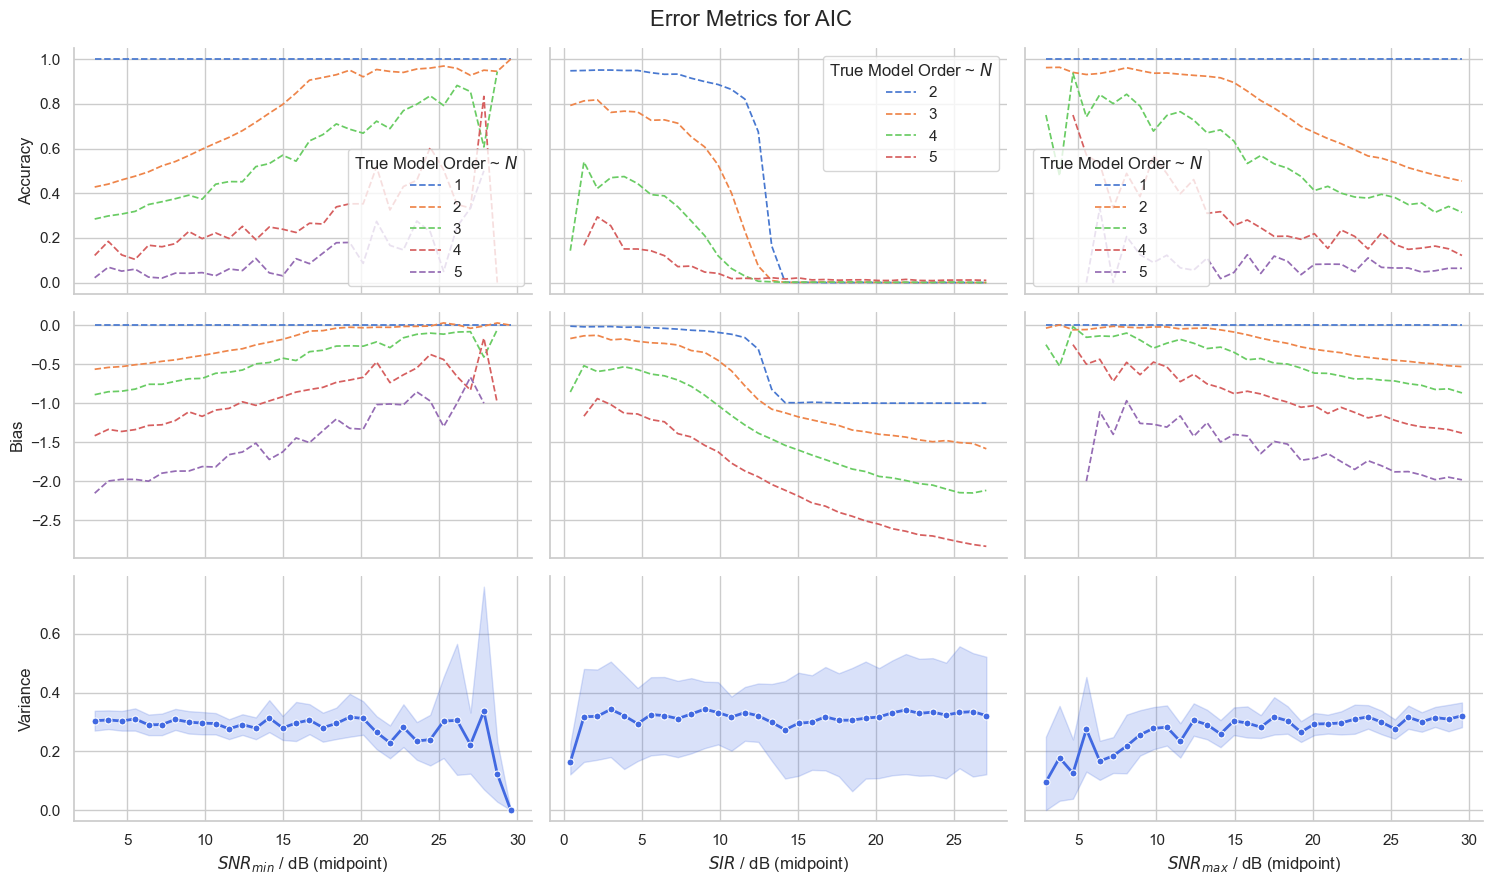
\includegraphics[width=\textwidth]{figures/07_Evaluation/snr_sir/aic_3x3.png}
    \caption{Accuracy, bias, and variance of the \gls{aic} given \( \SNRmin \), \( \SIR \) \& \( \SNRmax \).}
    \label{fig:eval_grids/aic}
\end{figure}
\begin{figure}[H]
    \centering
    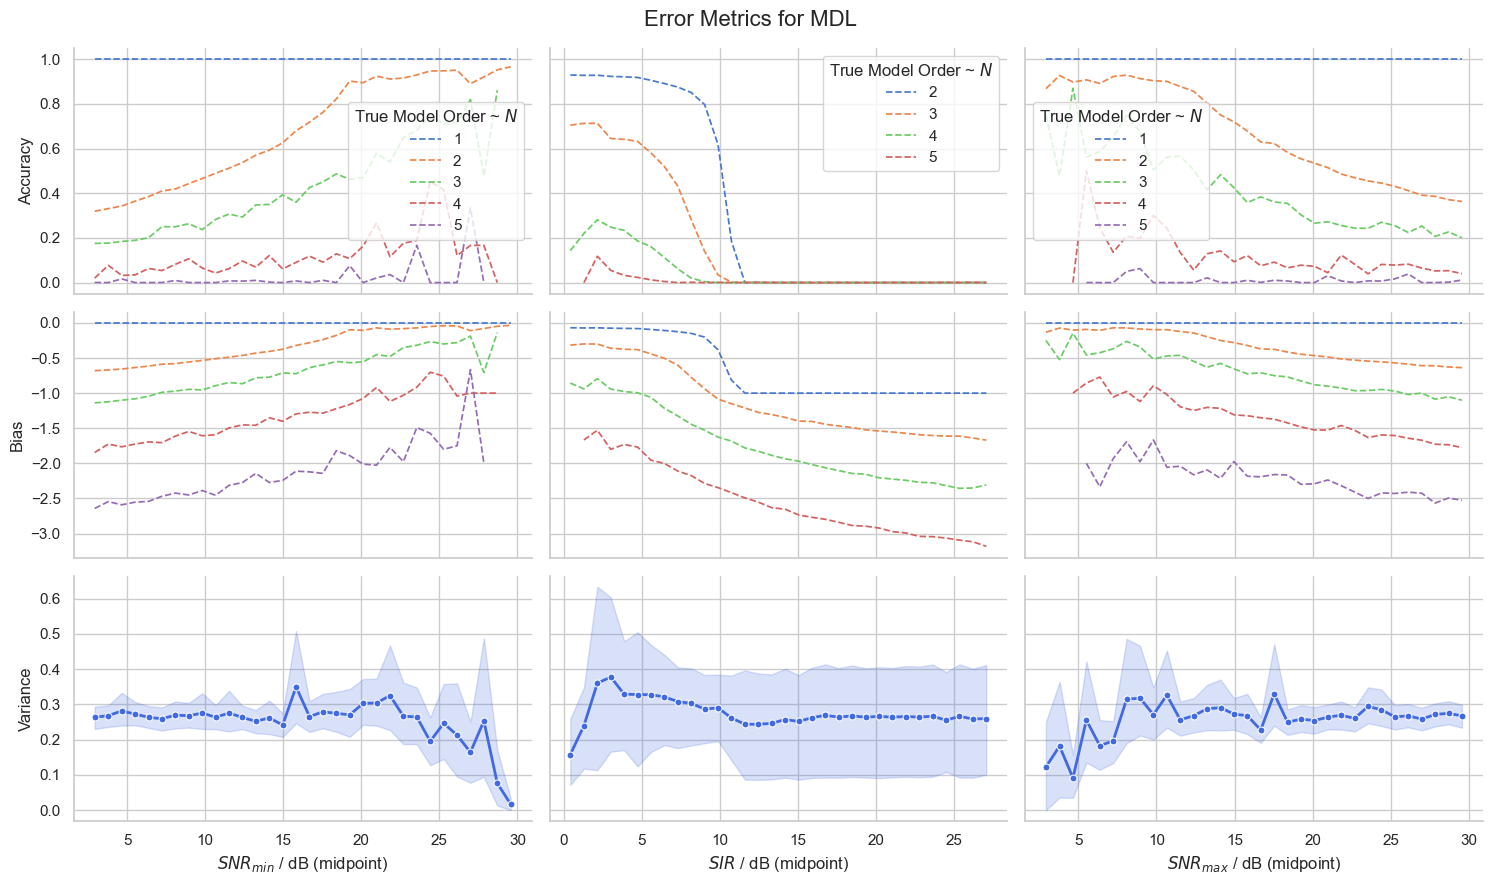
\includegraphics[width=\textwidth]{figures/07_Evaluation/snr_sir/mdl_3x3.png}
    \caption{Accuracy, bias, and variance of the \gls{mdl} given \( \SNRmin \), \( \SIR \) \& \( \SNRmax \).}
    \label{fig:eval_grids/mdl}
\end{figure}

Figures~\ref{fig:eval_grids/aic} and~\ref{fig:eval_grids/mdl} illustrate a strong negative correlation between the conventional
\glspl{ic}' bias and the \( \SIR \). \\
Once the \( \SIR \) exceeds \( 10 \si{\decibel} \), the accuracy of the \gls{mdl} plummets towards zero. The~\gls{aic} shows
analogue behavior with the drop occurring at \( \SIR = 15 \si{\decibel} \). \\
This trend can be observed more clearly in the figures~\ref{fig:aic_pred_hist} and~\ref{fig:mdl_pred_hist}.

\subsubsection{Neural Networks}
\begin{figure}[H]
    \centering
    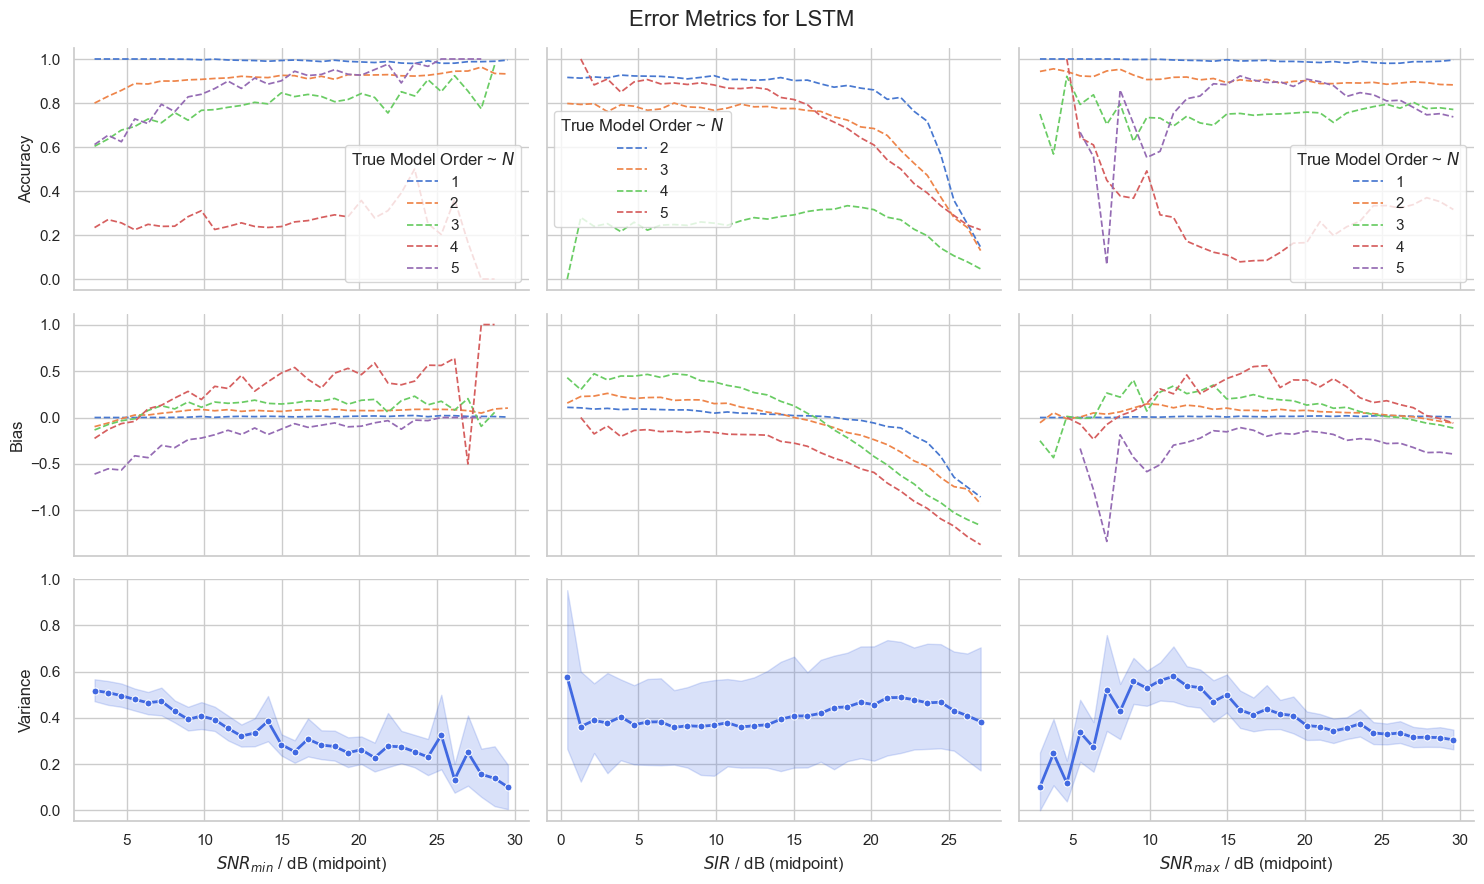
\includegraphics[width=\textwidth]{figures/07_Evaluation/snr_sir/lstm_3x3.png}
    \caption{Accuracy, bias, and variance of the \gls{lstm} given \( \SNRmin \), \( \SIR \) \& \( \SNRmax \).}
    \label{fig:eval_grids/lstm}
\end{figure}
\begin{figure}[H]
    \centering
    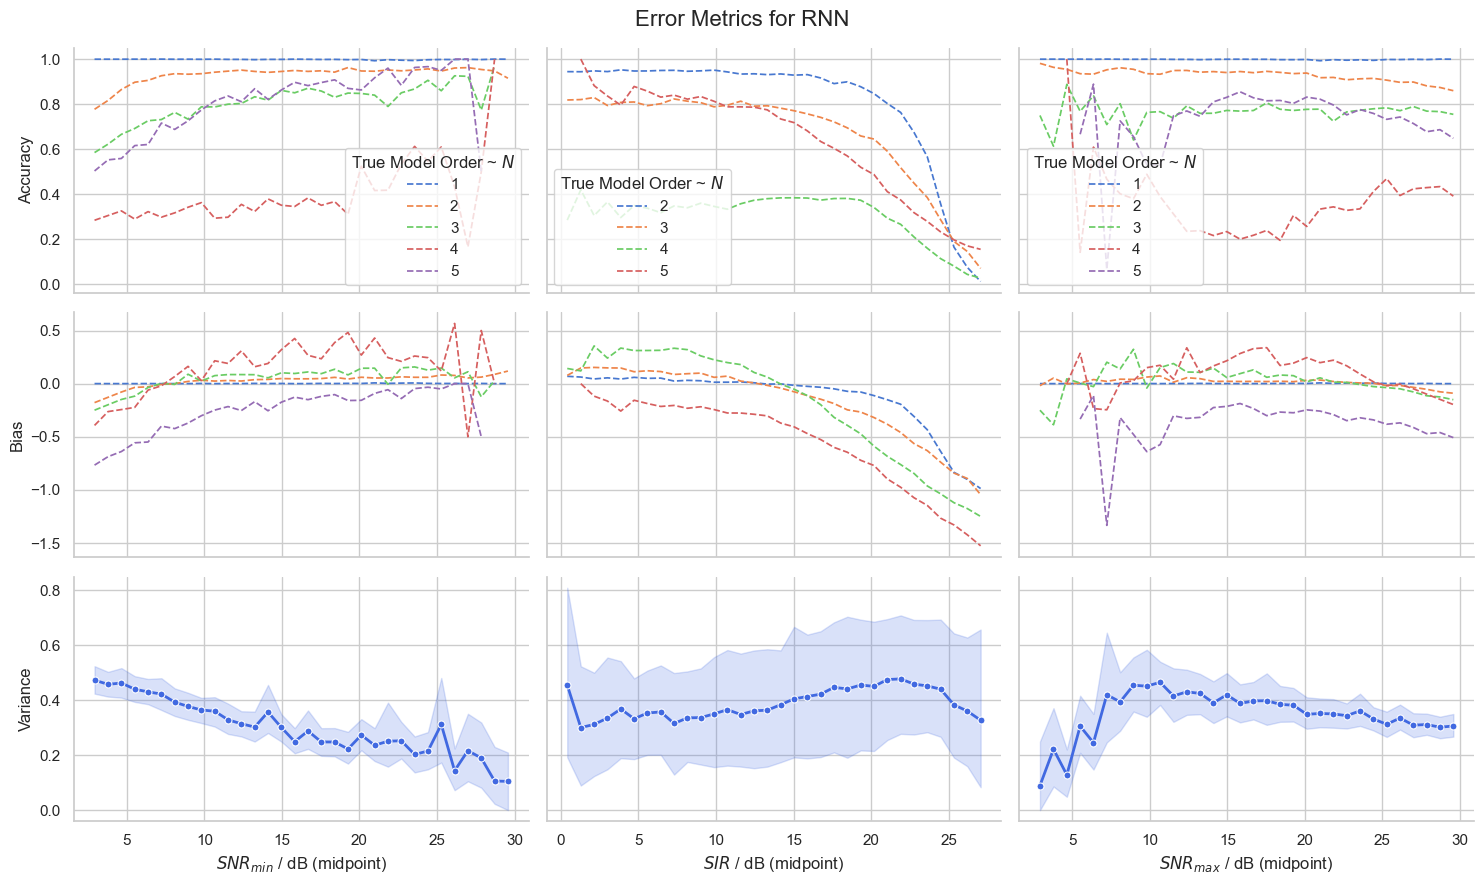
\includegraphics[width=\textwidth]{figures/07_Evaluation/snr_sir/rnn_3x3.png}
    \caption{Accuracy, bias, and variance of the \gls{rnn} given \( \SNRmin \), \( \SIR \) \& \( \SNRmax \).}
    \label{fig:eval_grids/rnn}
\end{figure}
\begin{figure}[H]
    \centering
    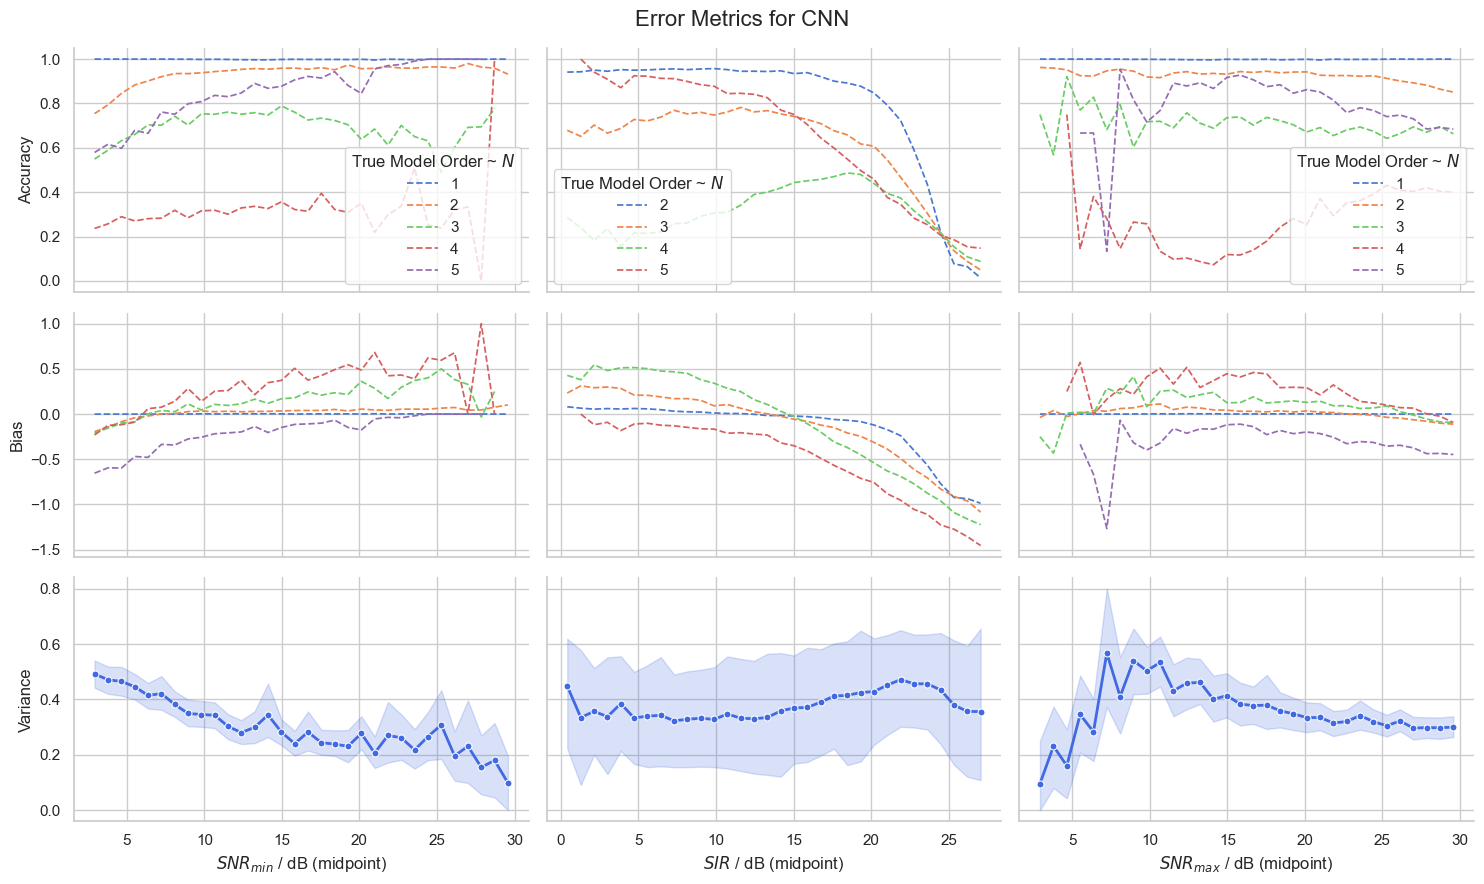
\includegraphics[width=\textwidth]{figures/07_Evaluation/snr_sir/cnn_3x3.png}
    \caption{Accuracy, bias, and variance of the \gls{cnn} given \( \SNRmin \), \( \SIR \) \& \( \SNRmax \).}
    \label{fig:eval_grids/cnn}
\end{figure}
\begin{figure}[H]
    \centering
    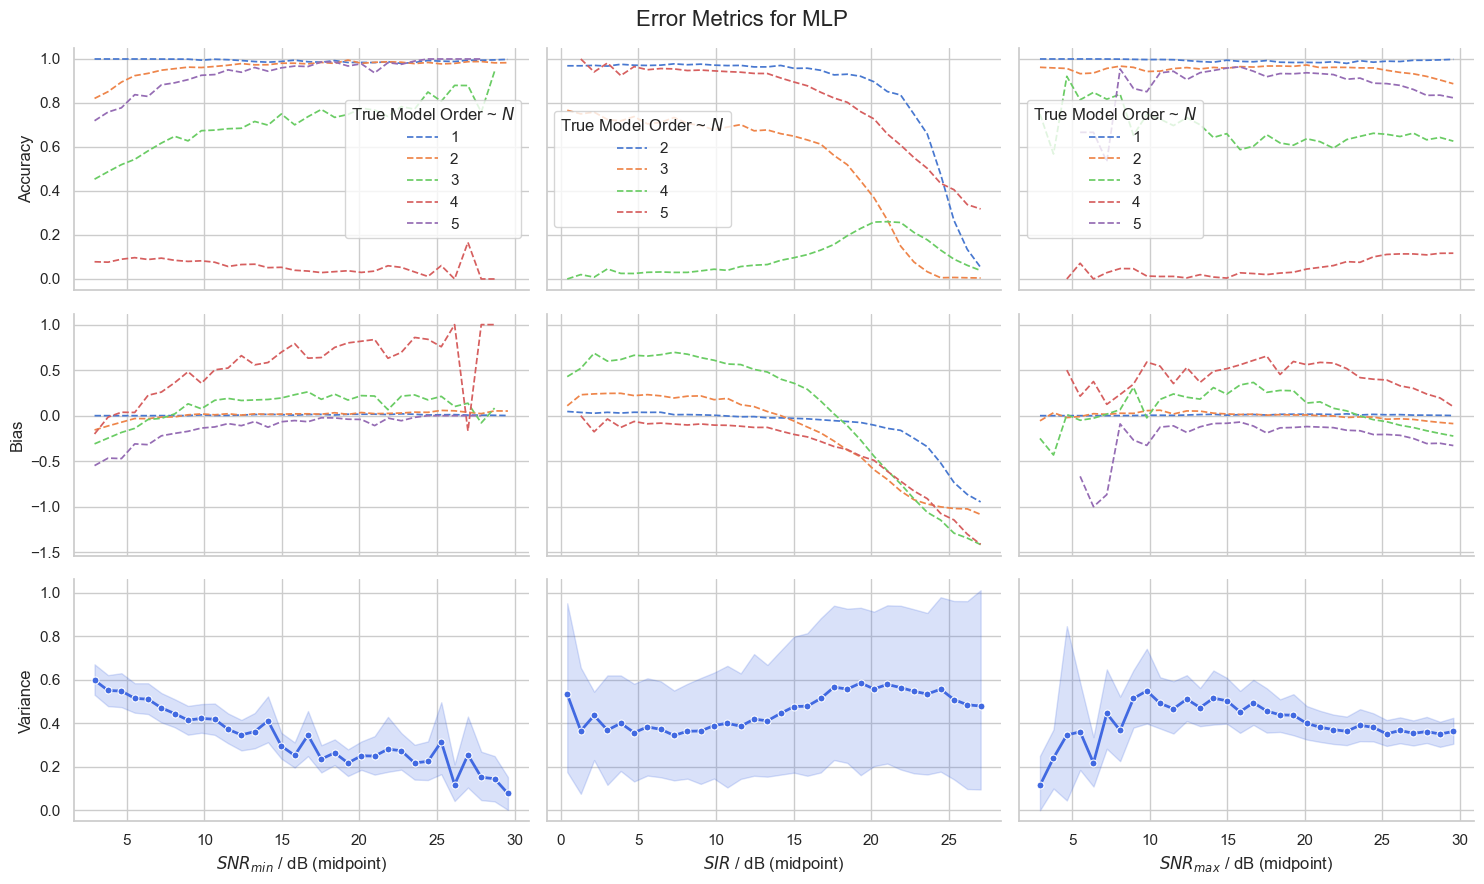
\includegraphics[width=\textwidth]{figures/07_Evaluation/snr_sir/mlp_3x3.png}
    \caption{Accuracy, bias, and variance of the \gls{mlp} given \( \SNRmin \), \( \SIR \) \& \( \SNRmax \).}
    \label{fig:eval_grids/mlp}
\end{figure}

It is an interesting observation that the accuracies and biases of all neural networks for \( N = 5 \) exhibit a
clear correlation with the \( \SNRmax \). This can be interpreted as evidence in favor of the hypothesis
\( \mathcal{H}_a \) in~\autoref{eq:pred_hypothesis}, as \( \mathcal{H}_0 \) does not explain any correlation between
the prediction likelihoods and any of the examined parameters of the signal model. \\
Considering that no complementary trend to this behavior can be observed when analyzing the variance with respect to the
\( \SNRmax \), it is reasonable to assume that the variance of the neural networks is directly influenced by the
\( \SNRmin \) instead of this effect being a result of the model order \( N \).

The visible negative correlation between the \( \SNRmin \) and the variance of the neural networks for all model orders \( N \)
might just be a result of the decreasing density of samples with higher \( N \) for increasing \( \SNRmin \). \\

Another clear trend is the increasing bias towards underestimating the model order with increasing \( \SIR \).
This observation is in line with intuition, as the increasing \( \SIR \) leads to a more pronounced distinction between
individual signal eigenvalues, which outshines the relative gap to the noise eigenvalues \( \bfL_{\eta} \).
Considering that even samples with \( N \in \{4,5\} \) display a bias which is negatively correlated with the \( \SIR \), counts as
another indicator in favor of \( \mathcal{H}_a \) in~\autoref{eq:pred_hypothesis}.

The unimodal trajectory of all variances with respect to the \( \SNRmax \) cannot be explained.


\section{Loss of positive definiteness}
The loss information about the underlying model order seems to arise continuously with a decreasing value of the smallest
eigenvalue \( \widehat{\lambda}_{\min} \) of the sub-sampled covariance matrix \( \C \). \\
As argued in~\cite{barthelme21sub} the loss of positive definiteness seems to be closely related with the loss of information,
encoded in the eigenstructure of the covariance matrix \( \C \), as the subspace decomposition becomes increasingly flawed
with decreasing \( \widehat{\lambda}_{\min} \).

\begin{figure}[H]
    \centering
    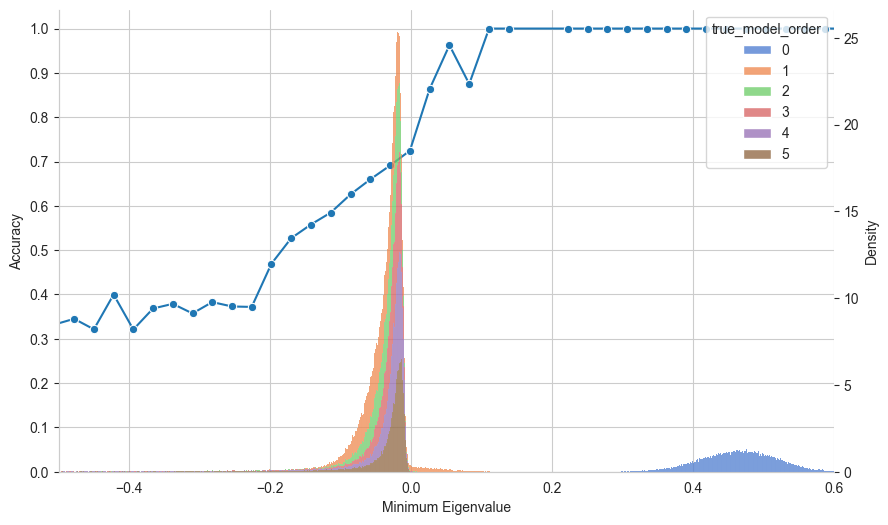
\includegraphics[width=0.6\textwidth]{figures/07_Evaluation/min_eigval/accuracy_ditrib.png}
    \caption{Mean accuracy of the neural networks superimposed with the PDF of \( \widehat{\lambda}_{\min} \).}
    \label{fig:min_eigval/accuracy_ditrib}
\end{figure}
\autoref{fig:min_eigval/accuracy_ditrib} shows the mean accuracy of the neural networks superimposed by the \gls{pdf} density
estimate of \( \widehat{\lambda}_{\min} \) evaluated on \( \DMain_{(\text{test})} \). \\
The displayed accuracy of an ensemble of \glspl{dnn} can be interpreted as a function of \( \widehat{\lambda}_{\min} \) that
quantifies the eigenvalues' ability to encode the coveted information about the underlying model order. \\

For reference, the \gls{pdf} of \( \widehat{\lambda}_{\min} \), evaluated on \( \DCoh \), is depicted in~\autoref{fig:min_eigval/pdf_min_eigval_coh}.
\begin{figure}[H]
    \centering
    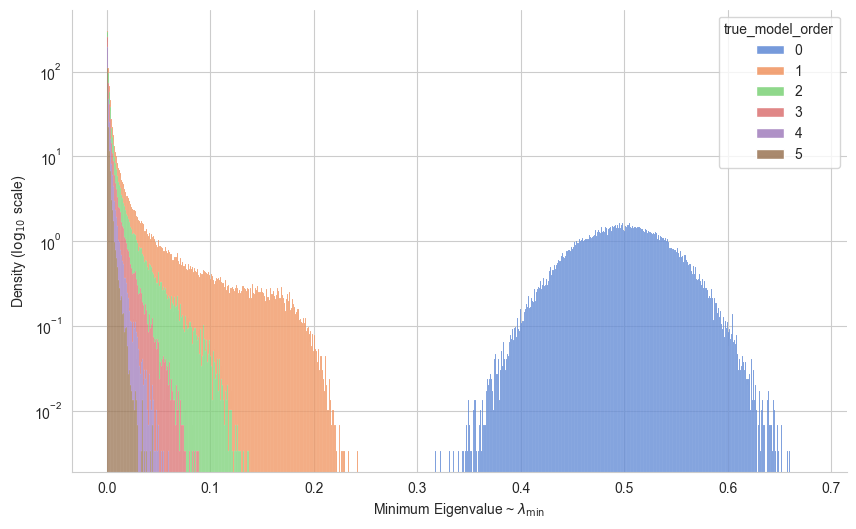
\includegraphics[width=0.6\textwidth]{figures/07_Evaluation/min_eigval/neg_eigvasls_distrib_coherent.png}
    \caption{PDF of \( \widehat{\lambda}_{\min} \) evaluated on \( \DCoh \).}
    \label{fig:min_eigval/pdf_min_eigval_coh}
\end{figure}
While the \gls{pdf} of \( \widehat{\lambda}_{\min} \), evaluated on \( \DCoh \), does not exhibit any negative eigenvalues
and shows a stronger differentiation between the smallest eigenvalues for different model orders \( N \), the distribution
of \( \widehat{\lambda}_{\min} \) does not align with the theoretical expectations as per~\autoref{eq:eigval_superimposed}.
The reason for this discrepancy is not clear at this point.

\begin{figure}[H]
    \centering
    \subfloat[]{{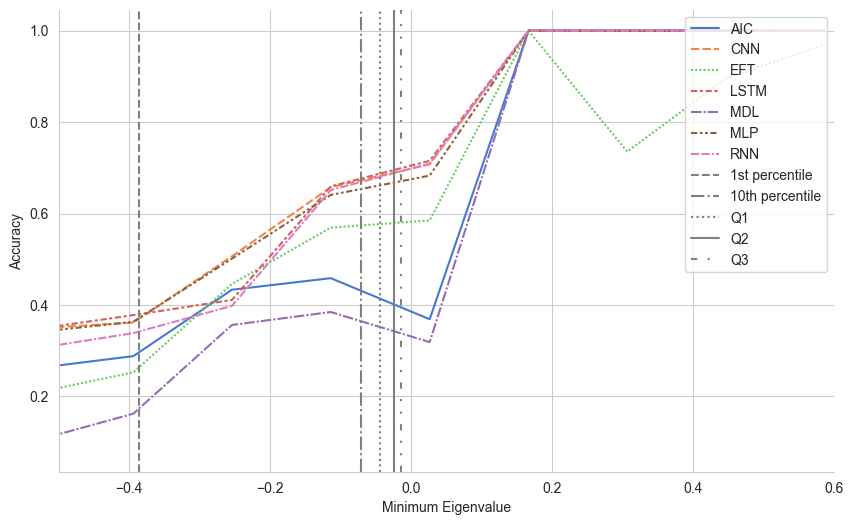
\includegraphics[width=0.5\textwidth]{figures/07_Evaluation/min_eigval/accuracy.png}}}
    \subfloat[]{{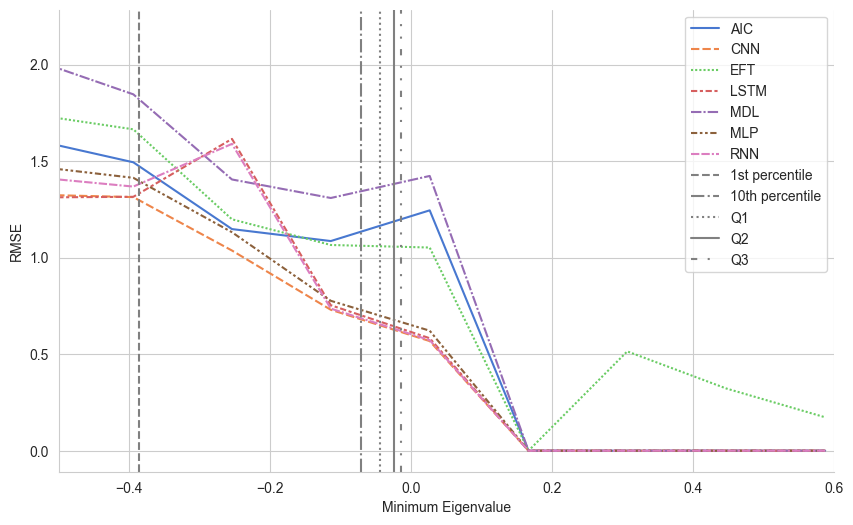
\includegraphics[width=0.5\textwidth]{figures/07_Evaluation/min_eigval/rmse.png}}}
    \caption{Accuracy (a) and RMSE (b) of the model order estimation methods vs.\ \( \widehat{\lambda}_{\min} \).}
    \label{fig:min_eigval/accuracy_rmse}
\end{figure}
\autoref{fig:min_eigval/accuracy_rmse} shows the mean accuracy and \gls{rmse} of each model order estimation method
against \( \widehat{\lambda}_{\min} \). \\
To allow a meaningful interpretation of the displayed results, the first three quantiles of the \( \widehat{\lambda}_{\min} \)
distribution are marked as vertical lines in the subplots. \\

\section{Influence of the number of snapshots}
\label{sec:influence_num_snapshots}

This section delves into the impact of the number of snapshots \( K \) on the performance of the various algorithms and
neural networks previously introduced. To allow this comparison we will utilize the \( \DKvar_{(\text{test})} \) dataset.
The evaluation on this dataset should be considered with caution, as not all methods had prior knowledge of the number of
snapshots \( K \) and / or were trained on \( \DKvar_{(\text{train})} \).
\begin{itemize}
    \item AIC, MDL, EFT, CNN+: Had prior knowledge of the number of snapshots \( K \).
    \item CNN (retrained), CNN+: Trained and tested on a \( 60:20:20 \) split of the dataset, and were thus tested on a subset of the full dataset.
    \item CNN, MLP, RNN, LSTM: Did not have prior knowledge of \( K \) and were trained on \( \DMain_{(\text{train})} \) with \( K = 100 \).
\end{itemize}

Notably, the \( [1,5] \) was unintentionally omitted from the subset used for training and testing CNN+ and CNN (retrained).

\autoref{fig:var_num_snapshots/accuracy} shows the mean accuracy of the neural networks and the \gls{moe} algorithms given
the number of snapshots \( K \) on the logarithmicly scaled x-axis.

\begin{figure}[H]
    \centering
    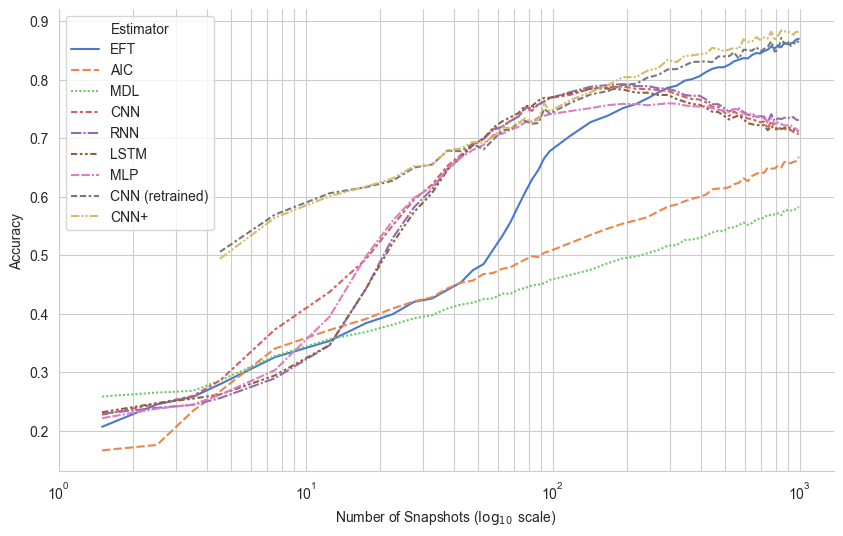
\includegraphics[width=0.8\textwidth]{figures/07_Evaluation/num_snapshots/accuracy+.png}
    \caption{Test accuracies of all model order estimation methods given the number of snapshots \( K \).}
    \label{fig:var_num_snapshots/accuracy}
\end{figure}

It is worth mentioning that all neural networks, which have not seen \( \DKvar \) during training, exhibit
a local optimum at around \( K = 200 \) snapshots.

All methods with prior knowledge or training on \( \DKvar_{(\text{test})} \) -- except for the \gls{eft} -- exhibit a
linear increase with respect to the logarithmicly scaled number of snapshots \( K \) on the x-axis.
This implies that the actual accuracies of these methods (\gls{aic}, \gls{mdl}, CNN+, and CNN (retrained)) are
exponentially increasing with respect to \( K \). This can also be seen as clear evidence for the assertion that the
incoherent covariance matrix \( \Csub \) indeed converges to the true covariance matrix-\( \Csub \rightarrow \bfm{C}_x \) as \( K \rightarrow \infty \),
which was claimed in~\cite{meyer}.

Furthermore, it is interesting to note that the \gls{eft} is on par with the \gls{aic} and \gls{mdl} for \( K < 50 \),
before its performance increases with a much more significant slope in the range \(50 \leq K \leq 100\) and subsequently
returns to its initial slope for \( K > 100 \), where it asymptotically converges to the performance of the neural networks
which have been trained on \( \DKvar_{(\text{train})} \).

The subtle advantage of the models which have only been exposed to \( \DMain \) around \( K = 100 \) is a strong indicator
that the two models which were trained on \( \DKvar_{(\text{test})} \) could benefit from further training on a slightly
larger dataset.


\begin{figure}[H]
    \centering
    \subfloat[]{{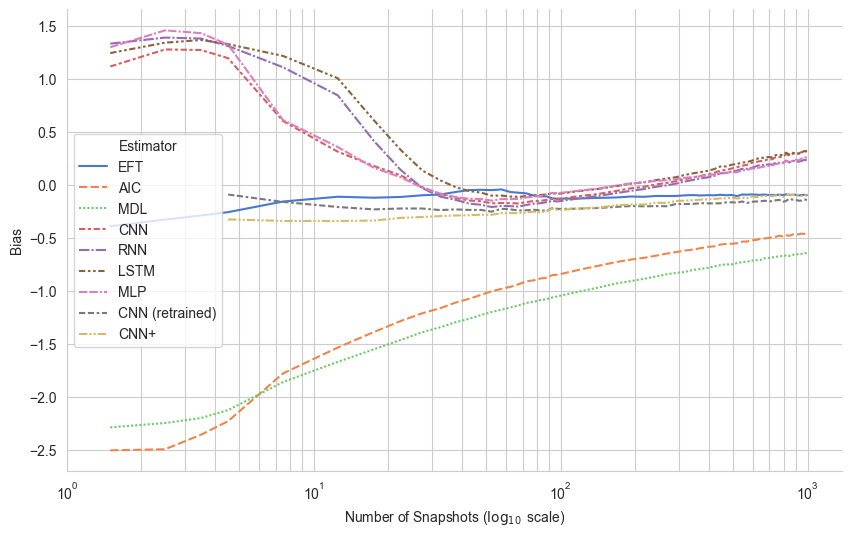
\includegraphics[width=0.5\textwidth]{figures/07_Evaluation/num_snapshots/bias+.png}}}
    \subfloat[]{{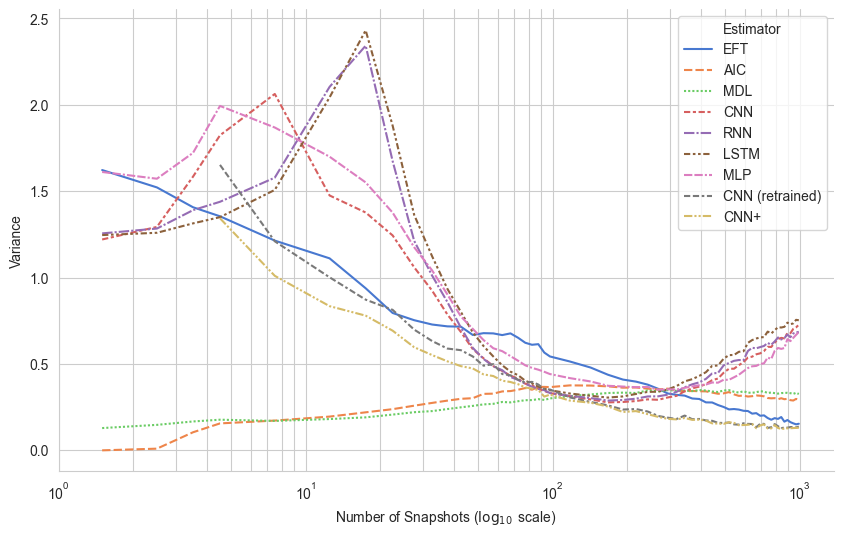
\includegraphics[width=0.5\textwidth]{figures/07_Evaluation/num_snapshots/variance+.png}}}
    \caption{Bias (a) and variance (b) of the model order estimation methods against the number of snapshots \( K \).}
    \label{fig:var_num_snapshots/bias_var}
\end{figure}

The overall low bias of CNN+ and CNN (retrained) is a strong indicator that the model complexity is sufficiently high
to capture the underlying relationships in the data, while still generalizing well to unseen data. Their bias seems
relatively stable across the entire range of \( K \).

While all networks which were solely trained on \( \DMain_{(\text{train})} \) exhibited a minor bias towards underestimating
the model order, they all tended to overestimation of the model order for \( K < 40 \), then a local minimum in terms
of bias around \( K \approx 60 \), where the bias is slightly negative, and a subsequent increase in bias for \( K > 60 \).

Most of the irreducible error of the neural networks seems to manifest in the variance, as the variance of the models which
were trained on \( \DKvar_{(\text{train})} \) exhibits a clear negative correlation with the number of snapshots.

The negative correlation between the variance and the number of snapshots \( K \) is a strong indicator


\section{Conclusion}

Although some evidence for the hypothesis \( \mathcal{H}_a \) in~\autoref{eq:pred_hypothesis} has been found, it does not
seem to be sufficient to draw any meaningful conclusion in favor of the employment of eigenvalue-based model order estimation
methods when the true model order \( N \) exceeds the number of RF chains. \\
